\documentclass[border=3mm]{standalone}
\usepackage{pgfplots}
\pgfplotsset{compat=newest}
\pagestyle{empty}
\begin{document}
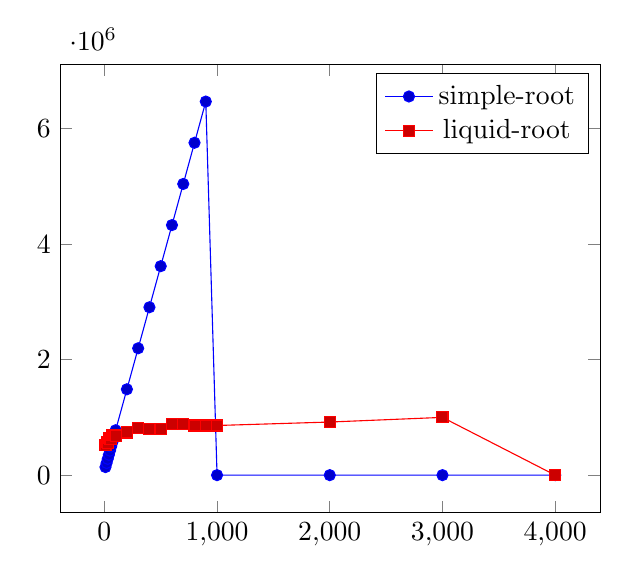
\begin{tikzpicture}
\begin{axis} 
\addplot  plot coordinates {
(10, 139758)
(20, 210619)
(30, 281487)
(40, 352360)
(50, 423240)
(60, 494126)
(70, 565018)
(80, 635916)
(90, 706821)
(100, 777732)
(200, 1487185)
(300, 2197263)
(400, 2907966)
(500, 3619294)
(600, 4331247)
(700, 5043826)
(800, 5757029)
(900, 6470857)
(1000, 0)
(2000, 0)
(3000, 0)
(4000, 0)
};\addplot  plot coordinates {
(10, 520250)
(20, 580441)
(30, 559707)
(40, 640301)
(50, 619823)
(60, 619695)
(70, 700354)
(80, 700354)
(90, 700418)
(100, 679812)
(200, 739737)
(300, 820587)
(400, 799789)
(500, 799917)
(600, 880448)
(700, 880384)
(800, 859906)
(900, 859906)
(1000, 859970)
(2000, 919895)
(3000, 1000554)
(4000, 0)
};\legend{simple-root,liquid-root}
\end{axis}
\end{tikzpicture}
\end{document}